 
\documentclass[10pt]{article}

\usepackage[slovak]{babel}
\usepackage[utf8]{inputenc}
\usepackage[T1]{fontenc}
\usepackage{graphicx}

\usepackage{times}


\usepackage[margin=1in]{geometry} 
\usepackage{amsmath,amsthm,amssymb}
 
\newcommand{\N}{\mathbb{N}}
\newcommand{\Z}{\mathbb{Z}}
 
\newenvironment{theorem}[2][Theorem]{\begin{trivlist}
\item[\hskip \labelsep {\bfseries #1}\hskip \labelsep {\bfseries #2.}]}{\end{trivlist}}
\newenvironment{lemma}[2][Lemma]{\begin{trivlist}
\item[\hskip \labelsep {\bfseries #1}\hskip \labelsep {\bfseries #2.}]}{\end{trivlist}}
\newenvironment{exercise}[2][Exercise]{\begin{trivlist}
\item[\hskip \labelsep {\bfseries #1}\hskip \labelsep {\bfseries #2.}]}{\end{trivlist}}
\newenvironment{reflection}[2][Reflection]{\begin{trivlist}
\item[\hskip \labelsep {\bfseries #1}\hskip \labelsep {\bfseries #2.}]}{\end{trivlist}}
\newenvironment{proposition}[2][Proposition]{\begin{trivlist}
\item[\hskip \labelsep {\bfseries #1}\hskip \labelsep {\bfseries #2.}]}{\end{trivlist}}
\newenvironment{corollary}[2][Corollary]{\begin{trivlist}
\item[\hskip \labelsep {\bfseries #1}\hskip \labelsep {\bfseries #2.}]}{\end{trivlist}}
 
\begin{document}
 
% --------------------------------------------------------------
%                         Start here
% --------------------------------------------------------------
 
%\renewcommand{\qedsymbol}{\filledbox}
 
\title{TIN - Domáca úloha č. 1}%replace X with the appropriate number
\author{Roman Dobiáš - xdobia11@stud.fit.vutbr.cz}
 
\maketitle

\section*{Úloha č.1}
\begin{enumerate}
\item 
    %%% 1 a) 
    \begin{proof}
    Nech $L_1, L_2 \in \mathcal{L}_3$. 
    Pomocou axiomu doplnku z teórie množín je možné previesť nasledujúcu úpravu:
        \begin{align*}
            L_1 \setminus L_2 = L_1 \cap \overline{L_2}
        \end{align*}
    Z vety 3.23 (skripta, str. 50) vieme, že trieda jazykov $\mathcal{L}_3$ je uzavretá voči
    $\cup$ a $\cap$ voči triede $\mathcal{L}_3$, a doplnku ku $\Sigma^{*}$.
            Nakoľko doplnok aj prienik sú uzavreté operácie v $\mathcal{L}_3$, potom $L_1 \cap
    \overline{L_2} \in \mathcal{L}_3$,a vzhľadom na úpravu potom aj $L_1 \setminus L_2 \in
    \mathcal{L}_3$. 
    \end{proof}
\item 
    %%% 1 b)    
    \begin{proof}
        Nech $L_1 \in \mathcal{L}_3, L_2 \in \mathcal{L}_2^D$. Z vety 4.27 (skriptá) vieme, že trieda
        $\mathcal{L}_2^D$ je uzavretá voči prieniku s jazykom triedy $\mathcal{L}_3^D$ a voči
        doplnku. 
        Preto $\overline{L_2} \in \mathcal{L}_2^D$ a zrejme $L_1 \cap \overline{L_2} \in
        \mathcal{L}_2^D$. Zároveň vieme, že $L_1$ aj $L_2$ sú množiny a platí pre ne vzťah $L_1
        \setminus L_2 = L_1\cap \overline{L_2}$. Preto nutne $L_1\setminus L_2 \in L_2^D$.
    \end{proof}

\item 
    %%% 1 c)    
    \begin{proof}
    Nech $L_1 = \Sigma^*$. Zjavne $L_1 \in \mathcal{L}_3$, kedže preň existuje deterministický konečný automat $M =
        (\{q_0\},\Sigma, \delta, q_0, \{q_0\})$, kde $\forall a \in \Sigma : \delta(q_0, a) = q_0$.
    Zároveň nech $L_2 \in \mathcal{L}_2$.

        Predpokladajme, že $\Sigma^* \setminus L_2 \in \mathcal{L}_2$. Potom nasledujúcou úpravou
        dostávame:
        \begin{align*}
            \Sigma^* \setminus L_2 = \{w | w \in \Sigma^* \land w \notin L_2 \} = \overline{L_2} 
        \end{align*}
        Z predpokladu $ \Sigma^* \setminus L_2 \in \mathcal{L}_2$ dostávame $\overline{L_2} \in
        \mathcal{L}_2$, čo je spor, pretože z uzáverových vlastností bezkontextových jazykov vieme,
        že $\overline{L_2} \notin \mathcal{L}_2$. Preto neplatí predpoklad a platí $L_1 \setminus L_2 \notin
        \mathcal{L}_2$.
    \end{proof}
\end{enumerate}
\section*{Úloha č.2}
    Nech $P = (\{q_0, q_1, q_2, q_3\}, \{0,1,2\}, \{a,Z\}, \delta, q_0, Z, \{q_3\})$ je deterministický zásobníkový automat, kde
    $\delta$ je definované nasledovne:
    \begin{align*}
        \delta (q_0, 1, Z) &= (q_0, aZ)  & \delta (q_0, 1, a) &= (q_0, aa)\\
        \delta (q_0, 2, Z) &= (q_0, aaZ) & \delta (q_0, 2, a) &= (q_0, aaa)\\
        \delta (q_0, 0, Z) &= (q_0, Z)   & \delta (q_0, 0, a) &= (q_0, a)\\
        \delta (q_0, \#, a) &= (q_1, a)   & \delta (q_0, \#, Z) &= (q_1, Z)\\
        \delta (q_1, a, a) &= (q_1, \epsilon) & \delta (q_1, b, a) &= (q_2, \epsilon)\\
        \delta (q_1, 0, a) &= (q_1, a)   & \delta (q_2, \epsilon, a) &= (q1, \epsilon)\\
        \delta (q_1, \epsilon, Z) &= (q3, \epsilon) & \delta (q_3, \epsilon, Z) &= (q_3, Z)\\
    \end{align*}
    Diagram výsledného automatu je znázornený na obrázku \ref{automata}. Výsledný DZA prijíma
    reťazec prechodom do koncového stavu a prečítaním celého vstupného reťazca.

\begin{figure}
    \label{automata}
    \centering
    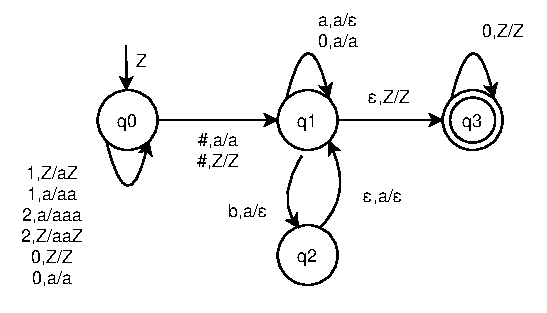
\includegraphics{dpda.pdf}
    \caption{Diagram DZA z úlohy č.2. Automat prijíma prechodom do koncového stavu.}
\end{figure}


\section*{Úloha č.3}
Dôkaz je prevedený pomocou Pumping Lemma. 
\begin{proof}
Predpokládajme, že jazyk L je nekonečným regulárnym jazykom. Potom existuje $k > 0$ a reťazec $w =
a^k\#a^k$ z jazyka L, pre ktorý platí $|w| = 2k+1$, teda $|w|\geq k$, a platí nasledujúce tvrdenie:
\begin{align*}
    \exists x,y,z \in (N \cup \Sigma)^*: w = xyz \land |xy| \leq k \land y \neq \epsilon : \forall i \in
    \mathbb{N}_0: xy^iz \in L 
\end{align*}
    Zvoľme ľubovoľné $l,n \in \mathbb{N}$ také, že platí $x = a^{n} \land y = a^{l} \land z =
    a^{k-l-n}\#a^k \land l > 0 \land n \geq 0 \land l+n \leq k$. Potom musí platiť, že $\forall
i \in \mathbb{N}_0: xy^iz \in L$.

Uvažujme prípad $i = 0$. Potom by podľa prepokladu malo platiť $xz \in L$, lenže zjavne platí
    $a^{n}a^{k-l-n}\#a^{k} = a^{k-l}\#a^{k} \notin L$, čo je v spore s predpokladom, že L je regulárny jazyk. Preto L nie je regulárny jazyk.
\end{proof}


\section*{Úloha č.4}

\textbf{Vstup:} Pravá lineárna gramatika $G_P = (N, \Sigma, P, S)$ taká, že $P$ obsahuje len pravidlá typu
$A\to xB, x \in (N\cup\Sigma)^*, A,B \in N$ a typu $A\to x, x \in (N\cup\Sigma)^*, A \in N$\\
\textbf{Výstup:} Ľavá lineárna gramatika $G_L = (N_1, \Sigma, P_1, S_1)$ taká, že $P$ obsahuje len pravidlá typu
$A\to Bx, x \in (N\cup\Sigma)^*, A,B \in N$ a typu $A\to x, x \in (N\cup\Sigma)^*, A \in N$\\
\textbf{Metóda:}
\begin{enumerate}
    \item $N_1 = N \cup \{S_1\}$
    \item Pre každé pravidlo z množiny $P$ typu $A\to xB, A,B \in N, x \in (N\cup\Sigma)^*$ pridaj
        do množiny pravidiel $P_1$ pravidlo:\\
        \begin{align*}
            B\to Ax
        \end{align*}
    \item Pre každé pravidlo z množiny $P$ typu $A\to x, A \in N, x \in (N\cup\Sigma)^*$ pridaj do
        množiny pravidiel $P_1$ pravidlo:\\
        \begin{align*}
            S_1\to Ax
        \end{align*}
    \item $P_1 = P_1 \cup \{S\to\epsilon\}$
\end{enumerate}

\subsection*{Demonštrácia algoritmu}
Pomocou vyžšie definovaného algoritmu predvedieme príklad transformácie gramatiky $G = (\{S,A,B\}, \{a, b\}, P, S),
P = \{S\to abA|bS, A\to bB|S|ab, B\to \epsilon | aA \}$:
\begin{enumerate}
    \item $N_1 = \{S, A, B\} \cup \{ S_1\}$
    \item $P_1$: 
            \begin{align*}
                A&\to Sab  & S&\to Sb\\
                B&\to Ab   & B&\to Ab\\
                S&\to A    & A&\to Ba
            \end{align*}
    \item $P_1$: 
            \begin{align*}
                S_1&\to Aab & S_1&\to B\epsilon
            \end{align*}
    \item $G_L = (N_1, \{a,b\}, P_1, S_1)$

\end{enumerate}

\section*{Úloha č.5}
Podľa Myhill-Nerudovej vety pre jazyk $L$ existuje deterministický konečný automat M taký, že $L(M)
= L$, práve vtedy ak prefixová ekvivalencia $\sim_L$ má konečný index. Budeme sa teda snažiť
dokázať, že jazyk $L$ má $\sim_L$ s konečným indexom.

\begin{proof}
Vzhľadom na predikát, ktorý určtuje príslušnosť daného reťazca do jazyka L, je možné definovať
    reláciu prefixovej ekvivalencie na jazyku L nasledovne:
\begin{align*}
u \sim_L v \iff \#_a(u)\bmod 3 = \#_a(v)\bmod 3 \land ((\#_b(u) > 0 \land \#_b(v) > 0) \lor (\#_b(u) = 0 \land
\#_b(v) = 0))
\end{align*}

Relácia $\sim_L$ nám definuje nasledujúce triedy rozkladu $\Sigma^* / \sim_L$:
\begin{align*}
    C_1 &= \{ w \in \Sigma^* | \#_a(w) \bmod 3 = 0 \land \#_b(w) = 0 \} & C_4 &= \{ w \in \Sigma^* | \#_a(w) \bmod 3 = 0 \land \#_b(w) > 0 \} \\
    C_2 &= \{ w \in \Sigma^* | \#_a(w) \bmod 3 = 1 \land \#_b(w) = 0 \} & C_5 &= \{ w \in \Sigma^* | \#_a(w) \bmod 3 = 1 \land \#_b(w) > 0 \} \\
    C_3 &= \{ w \in \Sigma^* | \#_a(w) \bmod 3 = 2 \land \#_b(w) = 0 \} & C_6 &= \{ w \in \Sigma^* | \#_a(w) \bmod 3 = 2 \land \#_b(w) > 0 \} \\
\end{align*}

Relácia $\sim_L$ rozdelí množinu $\Sigma^*$ na \textbf{6 tried ekvivalencie}. Počet tried vyplýva z
    počtu rôznych možností ohodnotenia funkcie $\#_a(x) \bmod 3$, ktorých je konečne, konkrétne 3, a faktu, že buď pre reťazec
    platí $\#_b(x) = 0$ alebo neplatí. Výsledný počet tried je daný počtom kombinácii oboch
    podmienok.   

Jazyk $L$ je zjednotením tried $C_5$ a $C_5$, pretože reťazce tíchto tried spĺňajú logickú formulu
z definície jazyka $L$, a teda náležia jazyku $L$. Zároveň má rozklad $\Sigma^* / \sim_L$ konečný
počet tried, teda relácia $\sim_L$ má konečný index a pre jazyk $L$ nutne existuje nejaký DKA taký,
že $L(M) = L$, teda jazyk $L$ je regulárny. 
\end{proof}
\newtheorem*{remark}{Poznámka}
\begin{remark}
DKA automat pre tento jazyk je znázornený na obrázku 2. Jednotlivé stavy automatu odpovedajú
    triedam rozkladu $\Sigma^* / \sim_L$.
\end{remark}
\begin{figure}[h!]
    \label{automata}
    \centering
    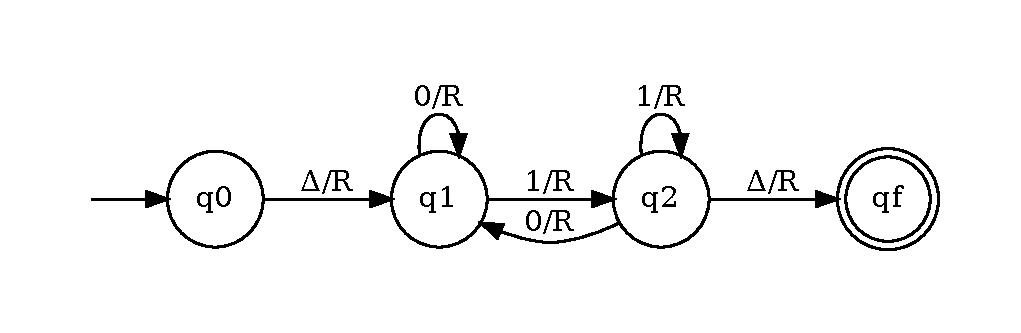
\includegraphics[height=6cm]{dfa.pdf}
    \caption{Diagram DFA z úlohy č.5.}
\end{figure}


\end{document}
